% !TEX TS-program = pdflatex
% !TEX encoding = UTF-8 Unicode
\documentclass[10pt]{article}

% amsmath package, useful for mathematical formulas
\usepackage{amsmath}
% amssymb package, useful for mathematical symbols
\usepackage{amssymb}
\usepackage[english]{babel}
% graphicx package, useful for including eps and pdf graphics
% include graphics with the command \includegraphics
\usepackage{graphicx}

% cite package, to clean up citations in the main text. Do not remove.
\usepackage{cite}

\usepackage{color} 

% Use doublespacing - comment out for single spacing
%\usepackage{setspace} 
%\doublespacing


% Text layout
\topmargin 0.0cm
\oddsidemargin 0.5cm
\evensidemargin 0.5cm
\textwidth 16cm 
\textheight 21cm

% Bold the 'Figure #' in the caption and separate it with a period
% Captions will be left justified
\usepackage[labelfont=bf,labelsep=period,justification=raggedright]{caption}

% Use the PLoS provided bibtex style
\bibliographystyle{plos2009}

% Remove brackets from numbering in List of References
\makeatletter
\renewcommand{\@biblabel}[1]{\quad#1.}
\makeatother


% Leave date blank
\date{}

\pagestyle{myheadings}
%% ** EDIT HERE **


%% ** EDIT HERE **
%% PLEASE INCLUDE ALL MACROS BELOW

%% END MACROS SECTION

\begin{document}

% Title must be 150 characters or less
\begin{flushleft}
{\Large
\textbf{Connectivity Analysis of Metagenomic Datasets}
}
% Insert Author names, affiliations and corresponding author email.
\\
Author1$^{ACH, JP, RCK, RM, ST, JJ, JMT, CTB}$, 
Author2$^{2}$, 
Author3$^{3,\ast}$
\\
\bf{1} Author1 Dept/Program/Center, Institution Name, City, State, Country
\\
\bf{2} Author2 Dept/Program/Center, Institution Name, City, State, Country
\\
\bf{3} Author3 Dept/Program/Center, Institution Name, City, State, Country
\\
$\ast$ E-mail: Corresponding author@institute.edu
\end{flushleft}

% Please keep the abstract between 250 and 300 words
\section*{Abstract}


\section*{Introduction}
Given the rapid decrease in the costs of sequencing, we can now achieve the sequencing depth necessary to study even the most complex environments \cite{Hess:2011p686,Qin:2010p189}.  High throughput, deep metagenomic sequencing efforts in permafrost soil, human gut, cow rumen, and surface water have provided insights into the genetic and biochemical diversity of environmental microbial populations \cite{Hess:2011p686,Iverson:2012p1281,Qin:2010p189} and the extent to which they are involved in responding to environmental changes \cite{Mackelprang:2011p1087}. These metagenomic studies have all leveraged \emph{de novo} metagenomic assembly of short reads to assign sequences to microbial taxa and function.  \emph{De novo} assembly is an advantageous approach to sequence analysis as it reduces the dataset size by collapsing numerous short reads into fewer contigs and provides longer sequences containing multiple genes and operons \cite{Miller:2010p226,Pop:2009p798} making annotation-based approaches more practical.  Furthermore, it does not rely on the availability of reference genomes to enable identification of novel genetic features and draft genomes \cite{Hess:2011p686,Iverson:2012p1281}.

Although \emph{de novo} metagenomic assembly is a promising approach for deep sequencing of metagenomes, it is complicated by the variable coverage of sequencing reads from mixed populations in the environment and their associated sequencing errors and biases \cite{Mende:2012p1262,Pignatelli:2011p742}. Several metagenomic-specific assemblers have been developed to deal with variable coverage communities, including Meta-IDBA \cite{Peng:2011p898}, MetaVelvet, and SOAPdenovo.  These assemblers rely on local models of sequencing coverage to help build assemblies and thus are sensitive to the effects of sequencing errors and biases on coverage estimations of the underlying dataset. The effects of sequencing errors on \emph{de novo} assembly has been demonstrated in simulated metagenomes \cite{Mavromatis:2006p894,Mende:2012p1262,Pignatelli:2011p742}, but these datasets do not incorporate models that are representative of real metagenomic data.  Specifically, these models exclude the presence of of known non-biological sequencing biases (\cite{GomezAlvarez:2009p1334,Keegan:2012p1336,Niu:2010p1333}) which would hinder coverage-based assembly approaches.  

In this study, we examine real metagenomic datasets for the presence of these artificial sequencing biases, extending previous work to large and complex datasets produced from the Illumina platform. Since these sequencing biases would erroneously connect numerous reads together, they can be characterized by their connectivity within an assembly graph.  Here, we take advantage of a de Bruijn assembly graph representation to identify and evaluate highly connective sequences within various metagenomic datasets.  We demonstrate that there exist highly connective sequences which originate, at least partially, from sequencing artifacts.  In metagenomic datasets, we find that the connectivity of these sequences limit approaches to divide or partition large datasets for further analysis, e.g. {de novo} assembly.  Here, we present approaches to identify and characterize these highly connective sequences and examine the effects of removing these sequences on downstream assemblies.

\section*{Results}

\subsection*{Connectivity analysis of metagenome datasets}

\subsubsection*{Presence of a single, highly-connected lump in all datasets}
We selected datasets from three diverse, medium to high diversity metagenomes from the human gut \cite{Qin:2010p189}, cow rumen \cite{Hess:2011p686}, and agricultural soil, representing metagenomes sequenced to various depths (Table 1, column 2).  To evaluate the effects of sequencing coverage, we included lower-coverage subsets of the soil metagenome (520 million reads) containing 50 and 100 million reads.  We also included a previously published error-free simulated, metagenome based on a mixture of 112 reference genomes \cite{Pignatelli:2011p742}.

Initially, we evaluated the amount of connectivity between all sequences in each metagenome using an approach similar to the initial step of short read assemblers to identify overlaps of short sequences of length 'k', or k-mers \cite{Peng:2011p898,Simpson:2009p233,Zerbino:2008p665}.  For complex metagenomes, extremely large diversity and numerous sequencing errors require large amounts of memory to store resulting assembly graphs \cite{Hess:2011p686,Mackelprang:2011p1087,Qin:2010p189}.  To overcome this limitation, we constructed a probabilistic representation of the assembly graph using a bloom filter de Bruijn graph representation within fixed memory as previously described (Pell et al, how to cite this?).  

Using this assembly graph representation, we separated reads contributing to disconnected portions of the metagenome assembly graph (e.g., representatives from separate populations in the source environment).  For each metagenome, regardless of origin, we found a single dominant, highly-connected set of sequencing reads which we henceforth refer to as the  "lump"  of the dataset (Table 1, column 3).  This lump contained the largest subset of connected sequencing reads and varied in size among the datasets, ranging from 5\% of total reads in the simulated metagenome to 75\% of total reads in the human gut metagenome.  For the soil datasets, as sequencing coverage (e.g., the fraction of reads mapped to an assembly) increased from 1.4 to 4.7 to 5.6\%, the lump size increased more dramatically from 7 to 15 to 35\% of all reads, indicating increasingly larger connectivity between sequences with more sequencing.

\subsubsection*{Characterizing the dominant lump within the assembly graph}

Given the large number of reads connected within metagenomic lumps (up to 182 and 262 million reads in the soil and human gut datasets, respectively), we quantified the degree of connectivity of sequences within the lump by estimating the average local graph density from nodes in the assembly graph (See Methods).  We observed that sequences in the identified metagenomic lumps had very high local graph densities, between 22 to 50\% of the total nodes in metagenomic lump assembly graphs had average graph densities greater than 20 (Table 1, column 8).  In comparison, 17\% of the total nodes in the simulated lump had an average local graph density greater than 20, and a mixture of the 112 source genomes for the simulated dataset had fewer than 2\% of its nodes with an average graph density greater than 20.  

We next assessed the extent to which graph density varied by position along the sequencing reads.  The degree of position-specific bias of graph densities was estimated by calculating the average local graph density within ten steps of every k-mer by position in each read.  In all environmental metagenomic reads, we observed biases in graph density at the 3'-end region of reads (Figure 1).  In soil metagenomes, we observed the most dramatic biases with estimated local graph density increasing at the 3'-end of the reads.  Notably, this bias was not present in the simulated dataset.  Next, we identified specific sequences within dense regions of the assembly graph which consistently contributed to high connectivity in an exhaustive graph traversal of the reads within each lump.  We observed that this subset of sequences were also found to exhibit position-specific biases within sequencing reads (Figure 1, solid lines).  Similar to local density trends, position-specific biases of these sequences also varied between metagenomes.  As sequencing coverage increased among metagenomes, the amount of 3'-end bias appeared to decrease (e.g., the soils) or inverse (e.g., rumen and human gut), and in the case of the simulated dataset, no such biases were observed.

\subsection*{Effects of removal of highly connective sequences on assembly}

In all datasets, we found that our approaches for removal of highly connective k-mers was effective at breaking apart metagenomic lumps and the resulting size of the largest partition of connected reads in each metagenome was reduced to less than 7\% of the total reads in the lump.  The partitioned sets of sequences could be assembled very efficiently in parallel, greatly reducing the memory and time required for assembly from greater than 100 GB and 100 hours (e.g. largest soil metagenome lump) to less than 2 GB memory  and less than 1 hour for all metagenomes.  

To explore the extent to which the identified highly-connective sequences impacted assembly, we first evaluated the effects of the removing these sequences from reads in the simulated lump and its resulting assemblies.  The assembly of the reads in the original, unfiltered simulated lump and that of the reads remaining after removing highly connective sequences (the filtered assembly) were compared for three assemblers (Velvet, Meta-IDBA, and SOAPdenovo).  Based on total assembly length of contigs greater than 300 bp, filtered assemblies of the simulated metagenome resulted in a loss of between 4 - 16\% of total assembly length (Table 2).   Filtered assemblies contained fewer total contigs than unfiltered assemblies, and the maximum contig size increased in the case of Velvet assembly but decreased in the case of the Meta-IDBA and SOAPdenovo assemblies.  Direct comparisons of the two assemblies found that the filtered assemblies comprised on average 88\% of the unfiltered assemblies, and the unfiltered assemblies contained nearly all (96\%) of the filtered assembled sequences.  Overall, despite the removal of over 3\% of the total unique 32-mers (Table 1) in the simulated metagenome, the resulting filtered assemblies resulted in only a loss of 0.1 - 0.6\% of annotated original reference genes (Table 2). 

We next evaluated the effects of using similar approaches on metagenomic datasets.  Similar to the simulated assemblies, the removal of highly connective sequences for all metagenomes and assemblers resulted in a loss of total assembly length and number of contigs (Table 2).  In general, filtered assemblies were largely contained within unfiltered assemblies and comprised 51-88\% of unfiltered assembly.   The observed changes in metagenomic assemblies were difficult to evaluate as the source genomes to these datasets are unknown, and a loss in assembly length may actually be beneficial due to the elimination of artifactual contigs.  To aid in this evaluation, we used the previously published set of rumen draft genomes which were constructed from \emph{de novo} assembly efforts of the rumen metagenome \cite{Hess:2011p686}.  Overall, we found that removal of highly connective sequences from the rumen dataset resulted in 1-3\% loss of sequences which matched to draft reference genomes.  

To further study the effects of highly connective sequences, we examined their incorporation into unfiltered assemblies.   Overall, less than 1\% of highly connective sequences on average were incorporated by any assembler, the maximum was 3-4\% in the Velvet and Meta-IDBA assemblies of the human gut dataset (Table 1 and 3).  Each assembled contig was divided into equal length bins (the size of bins was dependent on the total length of the contig) and examined for the presence of the previously identified highly connective sequences.  We found that contigs, especially in assemblies from Velvet and Meta-IDBA, incorporated a larger fraction of these sequences at its ends relative to other binned positions (Figure 3).  The SOAPdenovo assembler incorporated fewer of the highly connective sequences into its assembled contigs, none of these sequences in the simulated dataset were assembled and only 41 in the small soil dataset.  For the human gut metagenome assemblies, millions of the highly connective sequences were incorporated into assembled contigs, comprising nearly 4\% of all assembled sequences on Velvet contig ends (Supp. Fig. 1).

\subsubsection*{Characterizing highly connective sequences}

For the simulated metagenome, we could identify the original source of highly connective k-mers using available reference genomes.  Many of these sequences originated from well-conserved housekeeping genes involved in protein synthesis, cell transport, and signaling.  The top reference genes with perfect matches to highly connective k-mers which were present in the dataset a minimum of 50 times were identified (Table 4).  To determine possible biological sources of highly connective sequences within real metagenomes, we compared the sequences shared between the soil, rumen, and human gut metagenomes.  In total, 7,586 highly-connecting sequences (32-mers) were shared between the three soil, rumen, and human gut metagenomes.  We identified the closest reference protein from the NCBI-nr database requiring complete sequence identity.  Only 1,018 sequences (13\%) matched existing reference proteins, and many of the annotated sequences matched multiple conserved protein sequences from multiple genomes.  The top five proteins conserved in greater than 3 genomes are shown in Table 4, and largely encode for genes involved in protein biosynthesis, DNA metabolism, and biochemical cofactors (Table 5).

A potential cause of artificial high connectivity within metagenomes is the presence of high abundance sequences.  Thus, we identified the subset of highly connective k-mers which were also present with an abundance of greater than 50 within each metagenome and their location in sequencing reads (Figure 2, dotted lines).   These high abundance k-mers comprised a very small proportion of the identified highly connective sequences, less than 1\% in the soils, 1.5\% in the rumen, and 6.4\% in the human gut metagenomes, but the position-specific biases of these sequences were very similar to the biases of the larger set of highly connective k-mers.

To identify consistent patterns within sequences causing position-specific biases, we examined the abundance of distribution unique 5-, 6-, 7-, 8-mers contained within the high abundance subset of each dataset's highly connective k-mers. STILL FINISHING

\section*{Discussion}

\subsection*{Highly connected assembly subgraph contains sequencing artifacts}

Through assessing the connectivity of reads in several metagenomes, we identified a disproportionately large subset of reads which were connected together within an assembly graph, hereafter referred to as the "lump" in each metagenome.  The simulated metagenome's lump comprised 5\% of its total reads (Table 1).  As this dataset contains no errors, this observed connectivity represents conserved sequences within a single genome or between multiple genomes (Table 3).  In contrast, the highly connective lump within real metagenomic lumps comprised a significantly larger proportion of reads, ranging from 7\% to 75\% of the total reads (Table 1), suggesting that anomalous, non-biological connectivity may be present within these lumps.  Interestingly, in the soil metagenomes, we observed that the amount of connectivity nearly doubled with less than a 5\% increase of sequencing coverage.  When sequencing coverage increased slightly from 4.7 to 5.6\% in the medium and large soil metagenomes, the number of reads connected in the lump grew significantly from 15 million to 182 million.  Given the very high diversity and very low coverage of these soils, the magnitude of the observed increases in connectivity seemed unlikely from biological sources, further supporting the presence of sequencing biases within these datasets.  

If sequencing biases were present within these metagenomes, we would expect to observe that the metagenomic lumps would consist not only of artificial sequences but also sequences from reads which would be "preferentially attached" \cite{Barabasi:1999p1083}.  Consider that there is an original set of highly connecting "X" sequences in a lump.  These sequences would recruit a number of connective "Y" reads into the lump.  These recruited "Y" reads would then recruit more "Z" reads into the lump which would not necessarily connect to the original "X" reads.  In error-free datasets, we would observe this preferential attachment phenomenon as a linear increase of lump size with increasing sequencing coverage.  In the case of the presence of highly-connective sequencing biases, however, we'd observe that preferential attachment would cause dramatic increases in the number of recruited "Y" and "Z" reads, such is the observed case in the soil datasets.   

To more rigorously demonstrate the presence of artifacts within our datasets, we considered that the sequencing of metagenomes is a random process and thus any position-specific bias within sequencing reads is unexpected and non-biological.   For the metagenomes studied here, we used two approaches to examine characteristics of connectivity correlated to specific positions within sequencing reads.  First, we measured the local graph density (as defined in Methods) at specific positions within sequencing reads.  Next, we identified the specific k-mers which were consistently present in highly dense regions of the assembly graph and evaluated their location within sequencing reads.  When these approaches were applied to the simulated dataset, we observed no position-specific trends when assessing either local graph density (Figure 1) or highly connective k-mers (Figure 2, solid lines) as is consistent with the lack of sequencing errors and biases in this dataset.  In all real metagenomes, however, we identified position-specific trends in measurements of both local graph density and the location of highly connective sequences, clearly indicating the presence of artificial sequences.  Although present in all metagenomes, the direction of the bias varied between soil, rumen, and human gut datasets, particularly for the position-specific presence of highly connective sequences.  It is possible that in higher coverage datasets, such as the rumen and human gut, there is a larger presence of indirectly preferentially attached reads which are connected to high coverage sequences of biological origins.  This preferential attachment of such reads would result in increasing the number of total reads and consequently the decrease the total fraction of highly connective k-mers (Figure 2, y-axis).  This trend is observed in the decreasing fractions of highly connective sequences at the 3' end of reads as sequencing coverage increased in the small, medium, to large soil metagenomes and in the soil, rumen, to human gut metagenomes (Figure 2).

\subsection*{Effects of removing highly connective sequences on de novo assembly}

As is apparent from conserved biological sources of high connectivity within the simulated metagenome, not all the observed connectivity within real metagenomes is artificial, and our approaches are limited in that they cannot differentiate between sequencing artifacts and sources of real biological connectivity.  Regardless of the origin of highly connective sequences, we suspected that these sequences would challenge assemblers which rely on resolving the complex "lump" in the assembly graph.  Indeed, very few highly connective sequences with abundances greater than 50 were incorporated into any assembly (Table 3) and those which were assembled were disproportionately placed at the ends of contigs (Figure 3), suggesting that assembly could not extend beyond these sequences.  Although this trend was observed for all assemblers, it was more prevalent in the Velvet and Meta-IDBA assemblers, highlighting differences in assemblers.  

Given that these sequences were found to have position-specific biases within reads and challenged multiple assemblers, we removed them from metagenomic lumps.  The removal of these highly connective sequences had two key advantages:  firstly, it removed artificial sequences which should not be assembled, and secondly, it resulted in the dissolution of the high connectivity within the metagenomic lump and allowed for the partitioning of all metagenomes.  Having successfully divided metagenomic lumps, we compared the combined assembly of the partitioned sets of reads to the original lump dataset with several assemblers.  For the partitioned reads, we were able to assemble subsets of reads in parallel, resulting in significantly reduced assembly requirements (time and memory) (Table 2).  For the largest soil metagenome, containing over 500 million reads, we could not complete the Meta-IDBA assembly in less than 100 GB of memory.  After partitioning, the assembly could be completed in less than 2 GB of memory.  Additionally, we could use multiple k-mer length assemblies (demonstrated here with Velvet) and subsequently merge resulting assembled contigs, which was previously either impossible (due to memory requirements) or impractical (due to time).  In this study, we used consistent parameters for each assembler to compare unfiltered and filtered assemblies.  However, because the accuracy of an assembly relies on the characteristics of the underlying dataset, it is often beneficial to optimize assembly parameters and such optimization is much easier performed on assemblies which require less time and memory.  As metagenome dataset sizes grow increasingly larger, the ability to efficiently analyze partitioned datasets and/or evaluate multiple assemblies will be increasingly important.

The advantages of removing highly connective sequences must be balanced against consequences to resulting assemblies.  We compared several metagenome assemblies before and after the removal of these sequences.   Comparing the simulated dataset's assemblies, the removal of highly connective sequences resulted in very little loss of annotated reference genes and a similar assembly compared to the unfiltered data (~85\% similarity), supporting the removal of these highly connective sequences for more efficient assembly.  Unlike the simulated dataset, for the studied metagenomes, we compare filtered metagenomic assemblies against original assemblies of unknown quality.  For the rumen metagenome, we performed a partial evaluation of the assemblies using draft reference genomes previously constructed from the assembly of high abundance k-mers.   Similar to the simulated assemblies, we observed only a small loss of rumen reference genomes assembled (Table 2).  In general, for all metagenomes, we observed ~25\% loss in assembly after removing highly connective sequences, much more than observed in assemblies of reference genes and genomes in the simulated and rumen datasets.  Some of this loss is likely beneficial, resulting in the removal of sequencing artifacts; it is also possible that our approach removes sequences which can accurately be assembled but cannot be distinguished due to lack of reference genomes.  However, without the removal of these sequences, many of the assemblies of the larger metagenomes would not be as practical.  

\subsection*{Possible origins of highly connective sequences}

We attempted to identify any biological characteristics of highly connective sequences.  Among these sequences in the simulated dataset and those shared by all metagenomes, we identified a small fraction of these sequences (13\% in simulated and < 7\% in metagenomes) which matched reference genes, mostly associated with housekeeping functions (Tables 4 and 5).  Speculating that the remaining highly connective sequences originated from high abundance reads (both from biological sources of high connectivity or sequencing biases), we attempted to identify characteristics of the most abundant sequences.  We found that this subset (sequences which were present greater than 50x) displayed similar trends for position-specific biases compared to their respective sets of highly connective sequences (Figure 2), indicating that they are comprised of sequencing biases.  We attempted to identify signatures in the these sequences but found that they are largely random, making them difficult to efficiently identify and evaluate.  Currently, we are evaluating a promising approach to improve the identification and removal of probable sequencing artifacts based on targeting high abundance sequencing. 

\section*{Conclusion}

As datasets from NGS technologies continue to increase in size, our ability to analyze this sequencing data must reevaluated.  Here, we demonstrate the presence of sequencing artifacts within several metagenomic datasets that are a cause of non-biological connectivity within assembly graphs.  We show that these abundant, highly connective sequences are sources of sequencing artifacts in metagenomes and are difficult to assemble, regardless of their origin.  These sequences also add erroneous diversity and high coverage into metagenomes, significantly increasing memory requirements for de novo assembly.  Our previous efforts to resolve components of complex metagenome assembly graphs have been bottlenecked by the presence of these highly-connective sequences.  Here, we have developed approaches to identify these sequences and demonstrate that their removal results in comparable assemblies.  The removal of such sequences results not only in eliminating artificial sequences but also allows for the partitioning of disconnected subgraphs, significantly reducing assembly requirements.  Our analysis provides an understanding of the nature of these sequences and how their removal is an important first step for scalable \emph{de novo} assembly.  As datasets from NGS technologies continue to increase in size, this study highlights the importance of re-evaluating the nature of new sequencing data for both accurate and efficient downstream analysis approaches. 

\section*{Methods}

\subsection*{Metagenomic datasets}
All datasets, with the exception of the agricultural soil metagenome, originate from previously published datasets. Rumen-associated sequences (Illumina) were randomly selected from the rumen metagenome available at ftp://ftp.jgi-psf.org/pub/rnd2/Cow\_Rumen \cite{Hess:2011p686}. Human-gut associated sequences (Illumina) of samples MH0001 through MH0010 were obtained from ftp://public.genomics.org.cn/BGI/gutmeta/Raw\_Reads \cite{Qin:2010p189}.  The simulated high complexity, high coverage dataset was previously published (Pignatelli, 2011).  All reads used in this study, with the exception of those in simulated metagenome, were quality-trimmed for Illumina's read segment quality control indicator, where a quality score of 2 indicates that all subsequent regions of the sequence should not be used. After quality-trimming, only reads with lengths greater than 30 bp were retained. All quality trimmed datasets, including the previously unpublished agricultural soil metagenome, are available on a public Amazon EC2 snapshot, XXX. (temporarily on scratch hpc:/mnt/scratch/howead/to-transfer-to-amazon/.   The number of reads after quality-trimming is shown in Table 1 for each metagenome.  The sequencing coverage of each metagenome was estimated as the fraction of reads which could be aligned to assembled contigs with lengths greater than 500 bp.  For the coverage estimates, an assembly of each metagenome was performed using Velvet (v1.1.05) with the following parameters:  K=33, exp cov=auto, cov cutoff=0, no scaffolding.  Reads were aligned to assembled contigs with Bowtie (v0.12.7), allowing for a maximum of two mismatches.  

\subsection*{Lightweight, compressible de Bruijn graph representation}
We used a lightweight probabilistic de Bruijn graph representation to explore k-mer connectivity of the assembly graph (cite PNAS paper, software available at https://github.com/ctb/khmer). The de Bruijn graph stores k-mer nodes in Bloom filters and keeps edges between nodes implicitly, i.e. if two k-mer nodes exist with a k-1 overlap, then there is an edge between them. Bloom filters are a probabilistic set storage data structure with false positives but no false negatives, thus the size of the bloom filters were selected to be appropriate for each dataset and the memory available.  For analyzing the graph connectivity of the studied datasets, we used 4 x 48e9 bit bloom filters.  As metagenomic sequencing contains a mixture of multiple organisms, we could exploit the biological structure of the sequencing by partitioning the assembly graph into disconnected subgraphs that represent the original DNA sequence components. The set of the largest number of reads which were connected in the assembly graph is referred to above as a single, highly-connected lump.  Data and examples of scripts used for this analysis are available on the Amazon EC2 public snapshot:  data-in-paper/lumps and method-examples/0.partitioning-into-lump.

\subsection*{Local graph density and identifying highly-connected k-mers}
We implemented a systematic traversal algorithm to identify highly connected components of the assembly graph.  Waypoints were labeled to cover the graph such that they are a minimum distance of L apart. Originating from a waypoint, all k-mers (throughout the study k=32) were systematically and exhaustively traversed within a region that is the distance N.  The local graph density was calculated as the number of X k-mers reachable within a distance of N nodes (k-mers) divided by the distance N.  In this study, N was equal to 10 nodes within the assembly graph.  For the largest metagenomes, the metahit and large soil datasets, local graph density was calculated on a representative subset of reads due to computational limitations.  To identify specific highly-connective sequences within the lump assembly graphs, graph traversal to a distance of 40 nodes was attempted from marked waypoints.  If more than 200 k-mers were found within this traversal were identified, all k-mers within this traversal were identified as candidates for highly connective sequences.  If the same k-mers were consistently identified in other graph traversals, up to five times, the k-mer was flagged as a highly connective sequence.  Aligning theses k-mers to original sequencing reads, we identified the position-specific location of these k-mers.  Data and examples of scripts used for this analysis are available on the Amazon EC2 public snapshot: data-in-paper/density-bias, data-in-paper/hc-kmer-bias, method-examples/1.density-analysis, method-examples/2.identifying-hc-kmers, and method-examples/3.hc-kmer-analysis.

To identify the sources of highly connective k-mers identified in the simulated metagenome, these sequences were aligned against the reference genes originating from the 112 source genomes using Bowtie (v0.12.7) requiring exact matches.   Highly connective k-mers shared between all the metagenomes were also aligned against the NCBI non-redundant genome database (ftp://ftp.ncbi.nih.gov/blast/db, March, 1, 2011) using blastn \cite{Altschul:1990p1335} and requiring an exact match over the entire k-mer. 

We also identified the subset of highly connective k-mers which were present at greater than 50 times within lumps. Data used for this analysis are available on the Amazon EC2 public snapshot: data-in-paper/lumps/HC-kmers/HA-HC-kmers and method-examples/4.abundant-hc-kmers. These high abundance, highly connective sequences were also aligned to sequencing reads to demonstrate position specific biases.  We evaluated the existence of short k-mer (k=5-8) characteristics within high abundance, highly connective k-mers which did not have an exact match to the NCBI non-redundant database.  Each identified 32-mer was broken up into shorter k-mers, and the abundance of various k-mers was calculated.
  
\subsection*{\emph{De novo} Metagenomic Assembly}

To evaluate the effects of these k-mers on assembly, sequencing reads were trimmed at the location where a highly connective k-mer could be aligned and the resulting assemblies are referred to as "filtered" assemblies.  Untrimmed assemblies are referred to as "unfiltered" assemblies.  \emph{De novo} metagenomic assembly of reads within each unfiltered metagenomic lump was completed with Velvet (v1.1.02) with the following parameters: velveth -short -shortPaired (if applicable to the dataset) and velvetg -exp\_cov auto -cov\_cutoff 0 -scaffolding no \cite{Zerbino:2008p665}.  For the small and medium soil, rumen, and simulated datasets, Velvet assemblies were performed at K=25-49, resulting contigs were dereplicated to remove contigs with 99\% similarity using CD-HIT (v 4.5.6), and final contigs were merged with Minimus (Amos v3.1.0, \cite{Sommer:2007p1253}).  For the largest soil and human gut metagenomes, assemblies were performed at only K=33 due to the size of the datasets and memory limitations.  Additional assemblies were performed with meta-IDBA (v0.18) \cite{Peng:2011p898} : --mink 25 --maxk 50 --minCount 0 and with SOAPdenovo:  -K 31 -p 8  max\_rd\_len=200 asm\_flags=1 reverse\_seq=0.  After removal of highly connective k-mers in metagenomic lumps, each filtered lump was loaded into a new lightweight probabilistic de Bruijn graph representation to separate disconnected subgraphs.  Sequences in multiple subgraphs were grouped together such that assembly could be performed in parallel on each group of sequences.  Identical assembly parameters and methods as described above were performed on these partitioned sequences.  Unfiltered and filtered assemblies were compared using the total number of contigs, total assembly length, and maximum contig size.  Additional, the coverage of each assembly was calculated through estimating the average base pair coverage of the BLAST alignment of each assembly to one another (E-value > 10-5) or, in the case of the simulated and rumen assemblies, to reference genomes.  The simulated and rumen reference genomes were previously published in \cite{Hess:2011p686} and \cite{Pignatelli:2011p742}, respectively.  Data used for this analysis are available on the Amazon EC2 public snapshot: /data-in-paper/assembly*.

We examined the location of the identified high abundant, highly connecting k-mers within assembled contigs.  The location of these k-mers within assembled unfiltered contigs was examined by dividing each contig into 100 equally-sized regions.  The fraction of highly-connecting k-mers which aligned exactly to each region was calculated for each metagenome. Data and examples of scripts used for this analysis are available on the Amazon EC2 public snapshot: method-examples/5.hc-kmer-contigs/.


%\section*{References}

\bibliography{artifacts-bib}







\section*{Figures and Tables}

\begin{table}
\center{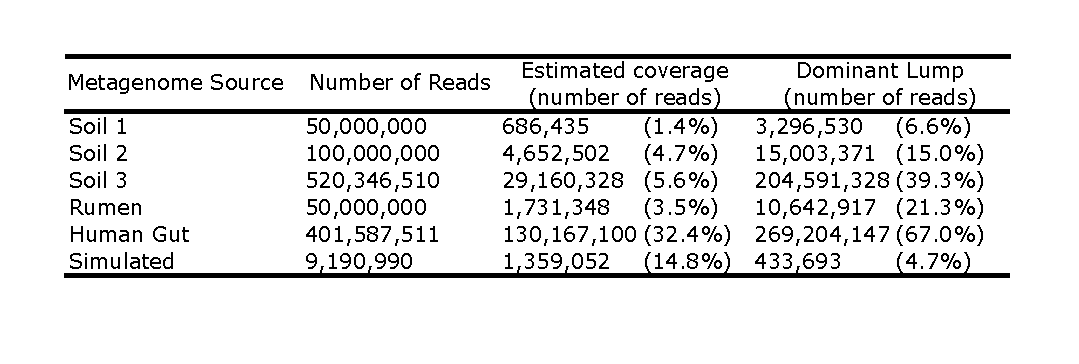
\includegraphics[width=5in]{./Figures/table1.pdf}}
\caption{The original size and proportion of highly connective 32-mers in the largest subset of partitioned reads ("lump") in several medium to high complexity metagenomes.  Read coverage was estimated with the number of aligned sequencing reads to Velvet-assembled contigs (K=33).  The dominant lump, or largest disconnected component of each metagenome assembly graph, was found to contain highly connecting k-mers responsible for high local graph density.}
\end{table}

\begin{table}
\center{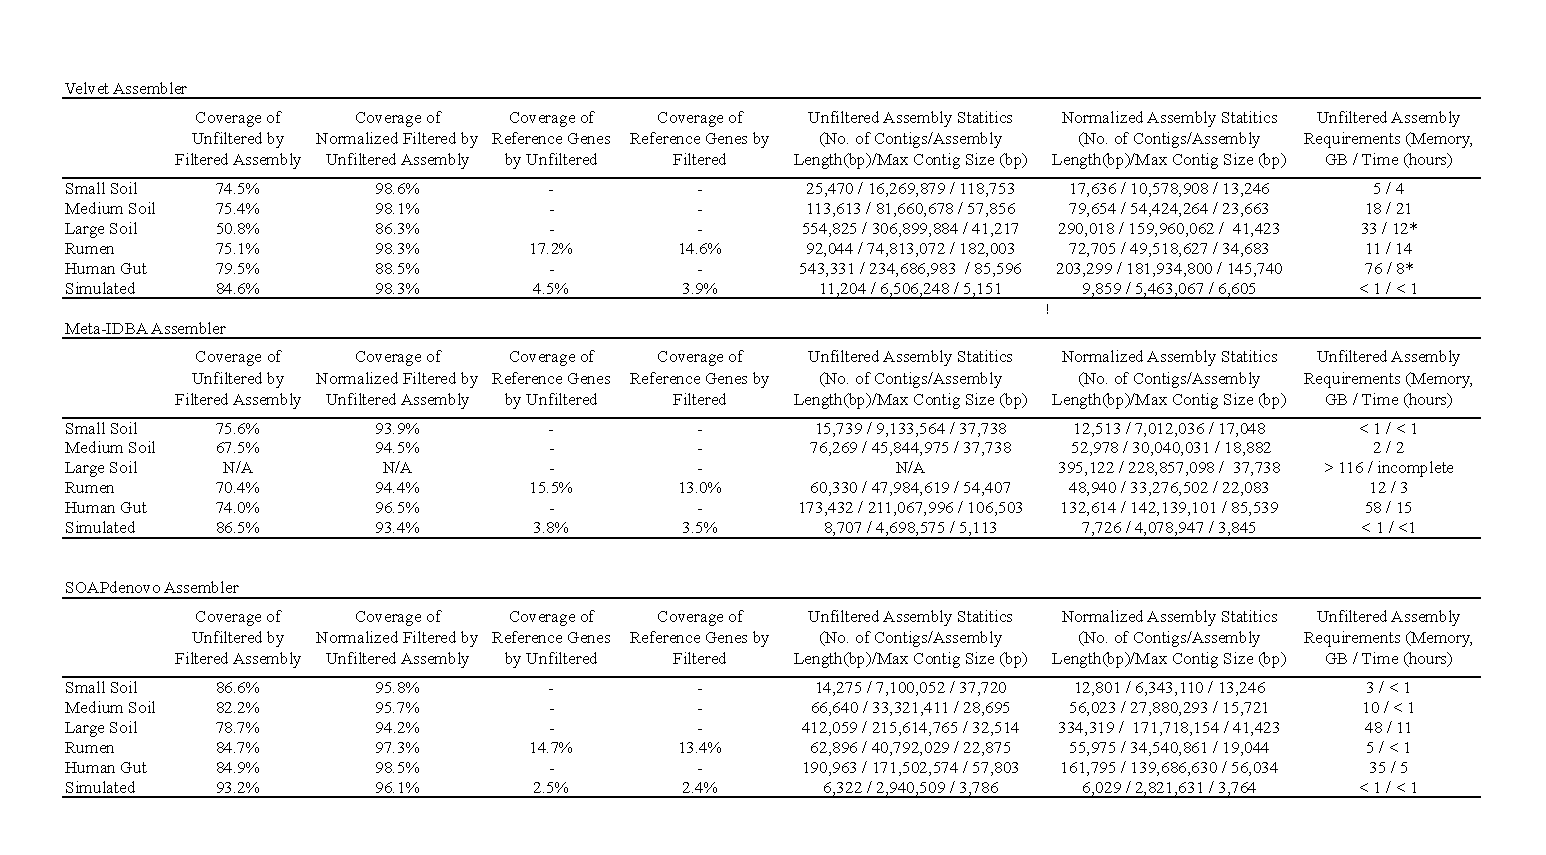
\includegraphics[width=5in]{./Figures/table2-assemblies.pdf}}
\caption{Comparison of unfiltered and filtered assemblies of various metagenome lumps using Velvet, SOAPdenovo, and Meta-IDBA assemblers.  Assemblies were aligned to each other, and coverage was estimated (columns 1-2).  Simulated and rumen assemblies were aligned to available reference genes/genomes (columns 3-4).  Total number of contigs, assembly length, and maximum contig size was estimated for each assembly, as well as memory and time requirements of unfiltered assembly (columnes 5-7).  Filtered assemblies required less than 2 GB of memory.  Velvet assemblies of the unfiltered human gut and large soil datasets (marked as *) could only be completed with K=33 due to computational limitations.  The Meta-IDBA assembly of the large soil metagenome could not be completed in less than 100 GB.}
\end{table}

\begin{table}
\center{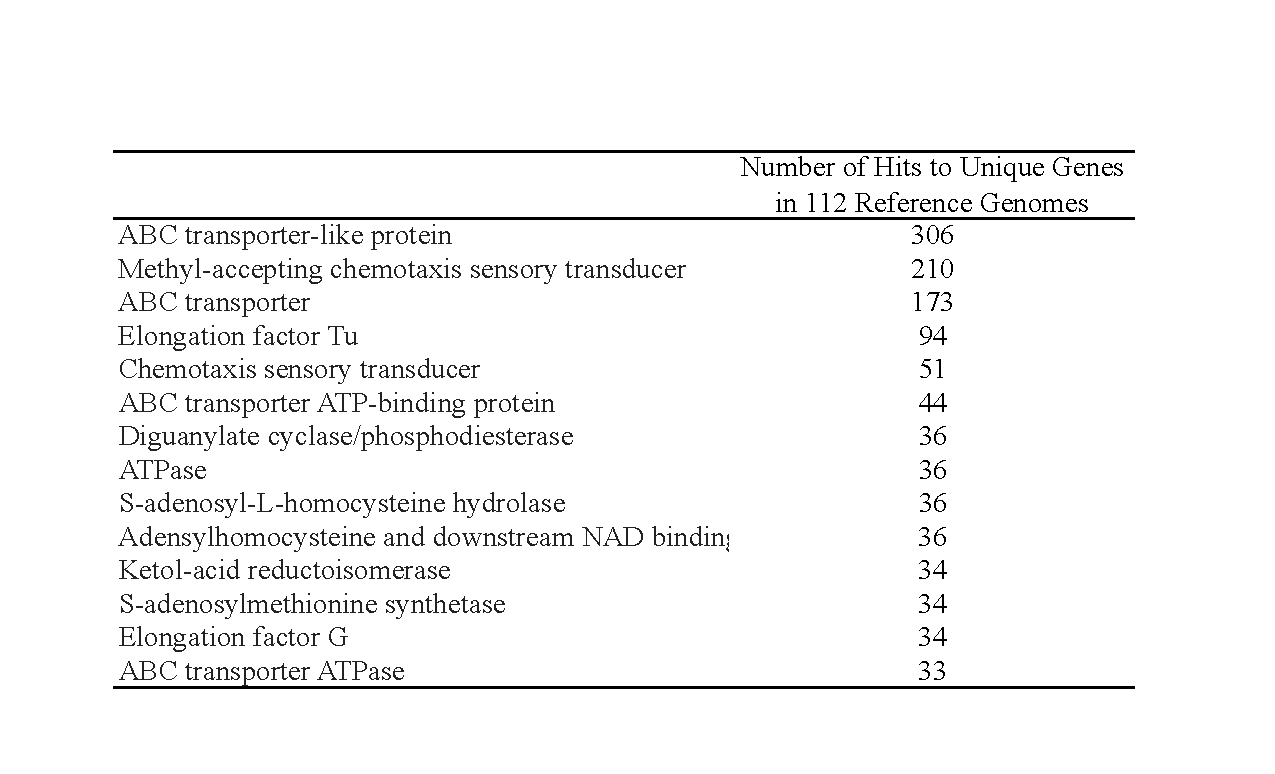
\includegraphics[width=5in]{./Figures/table3-simulated-stoptags.pdf}}
\caption{Annotation of highly-connecting sequences from the simulated metagenome with most hits to conserved genes within the 112 reference genomes \cite{Pignatelli:2011p742}.}
\end{table}

\begin{table}
\center{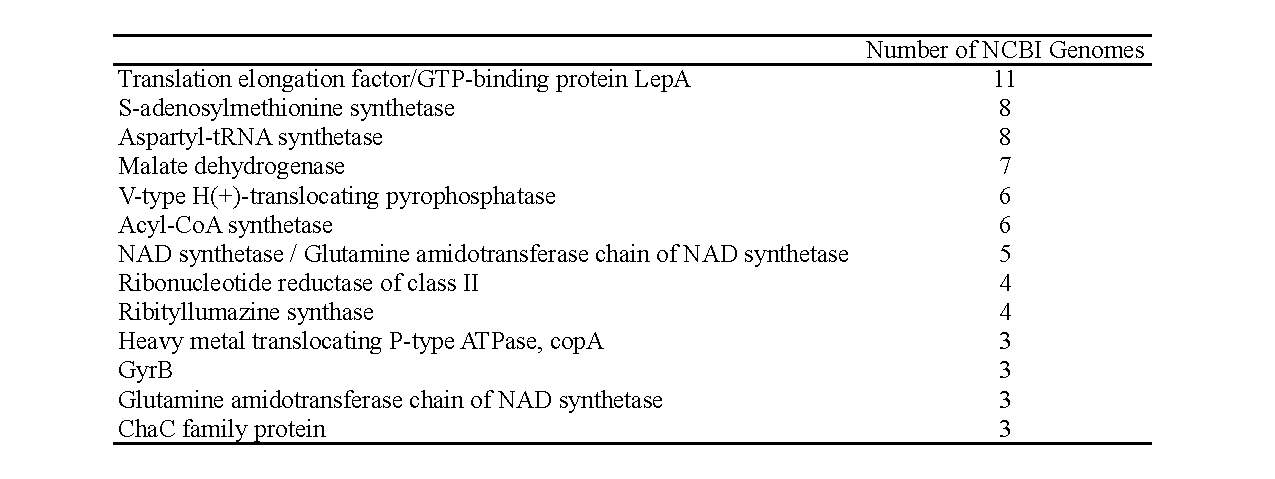
\includegraphics[width=5in]{./Figures/table4-overlap.pdf}}
\caption{Annotation of highly-connecting sequences to conserved nucleotide sequences originating from 3 or more reference genomes.  Shown are protein annotations whose nucleotide sequences matched 3 or more highly-connecting sequences shared in the three soil, rumen, and human gut metagenomes.}
\end{table}

\begin{figure}
\center{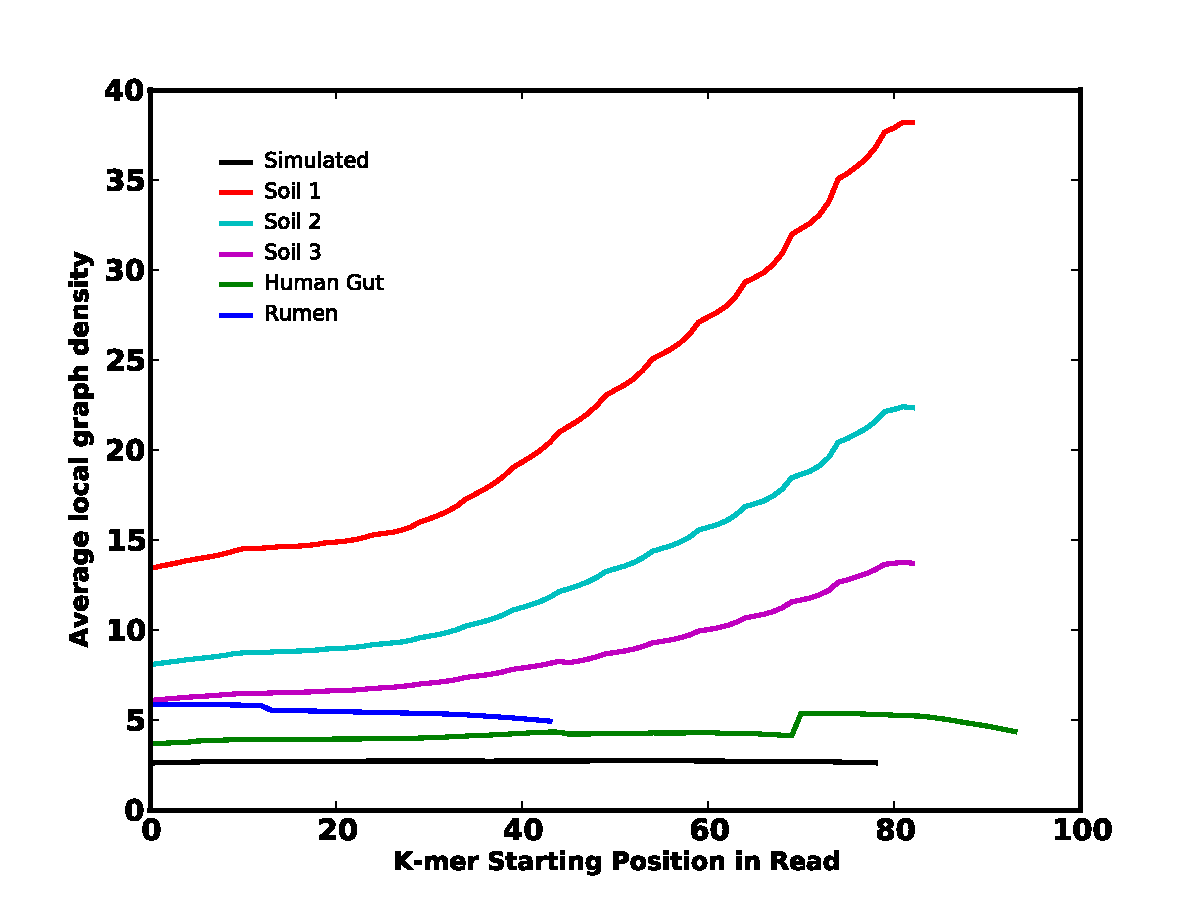
\includegraphics[width=5in]{./Figures/figure1-density.pdf}}
\caption{The extent to which average local graph density varies by read position is shown for the lump of various datasets.}
\end{figure}

\begin{figure}
\center{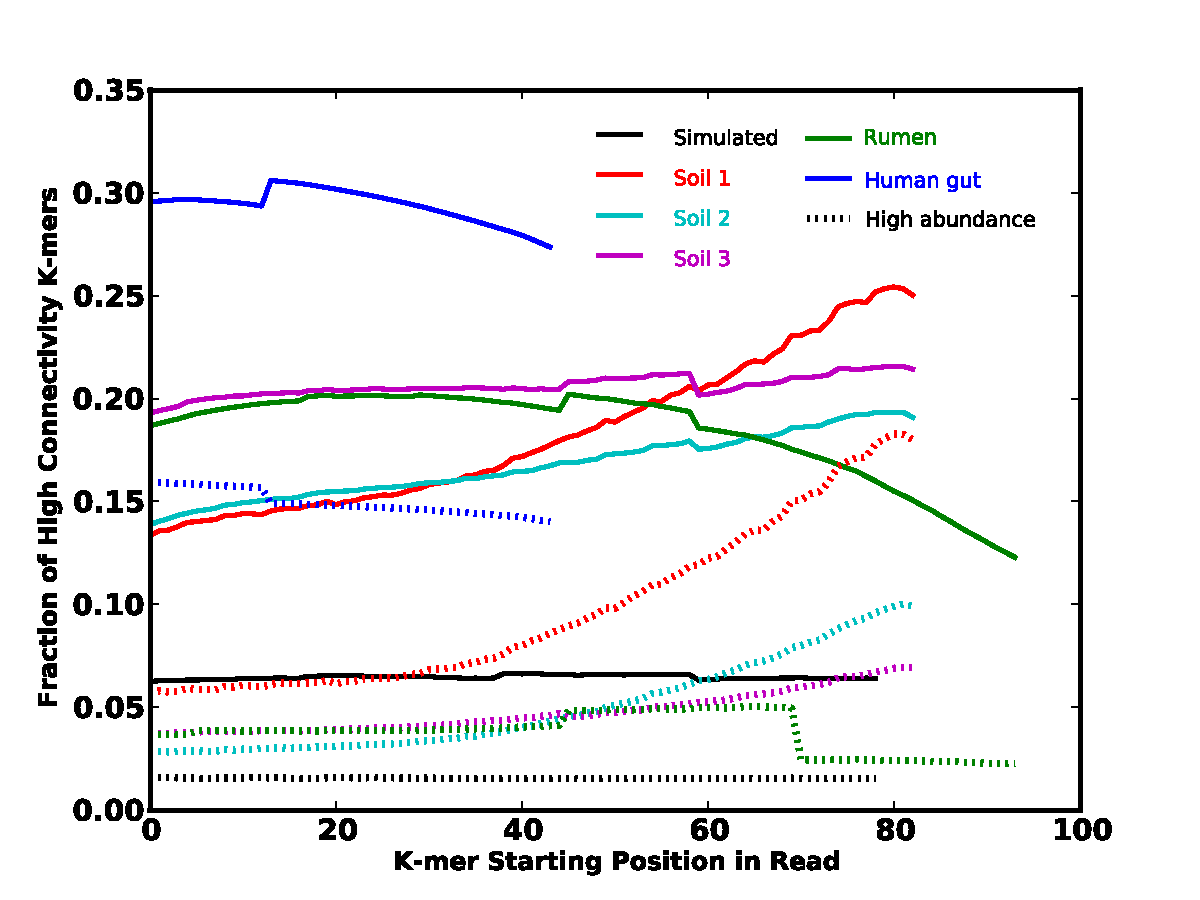
\includegraphics[width=5in]{./Figures/figure2-hckmers.pdf}}
\caption{The extent to which highly-connecting k-mers (solid lines) and the subset of highly abundant (greater than 50) k-mers (dashed lines) are present at specific positions within sequencing reads for various metagenomes.}
\end{figure}

\begin{figure}
\center{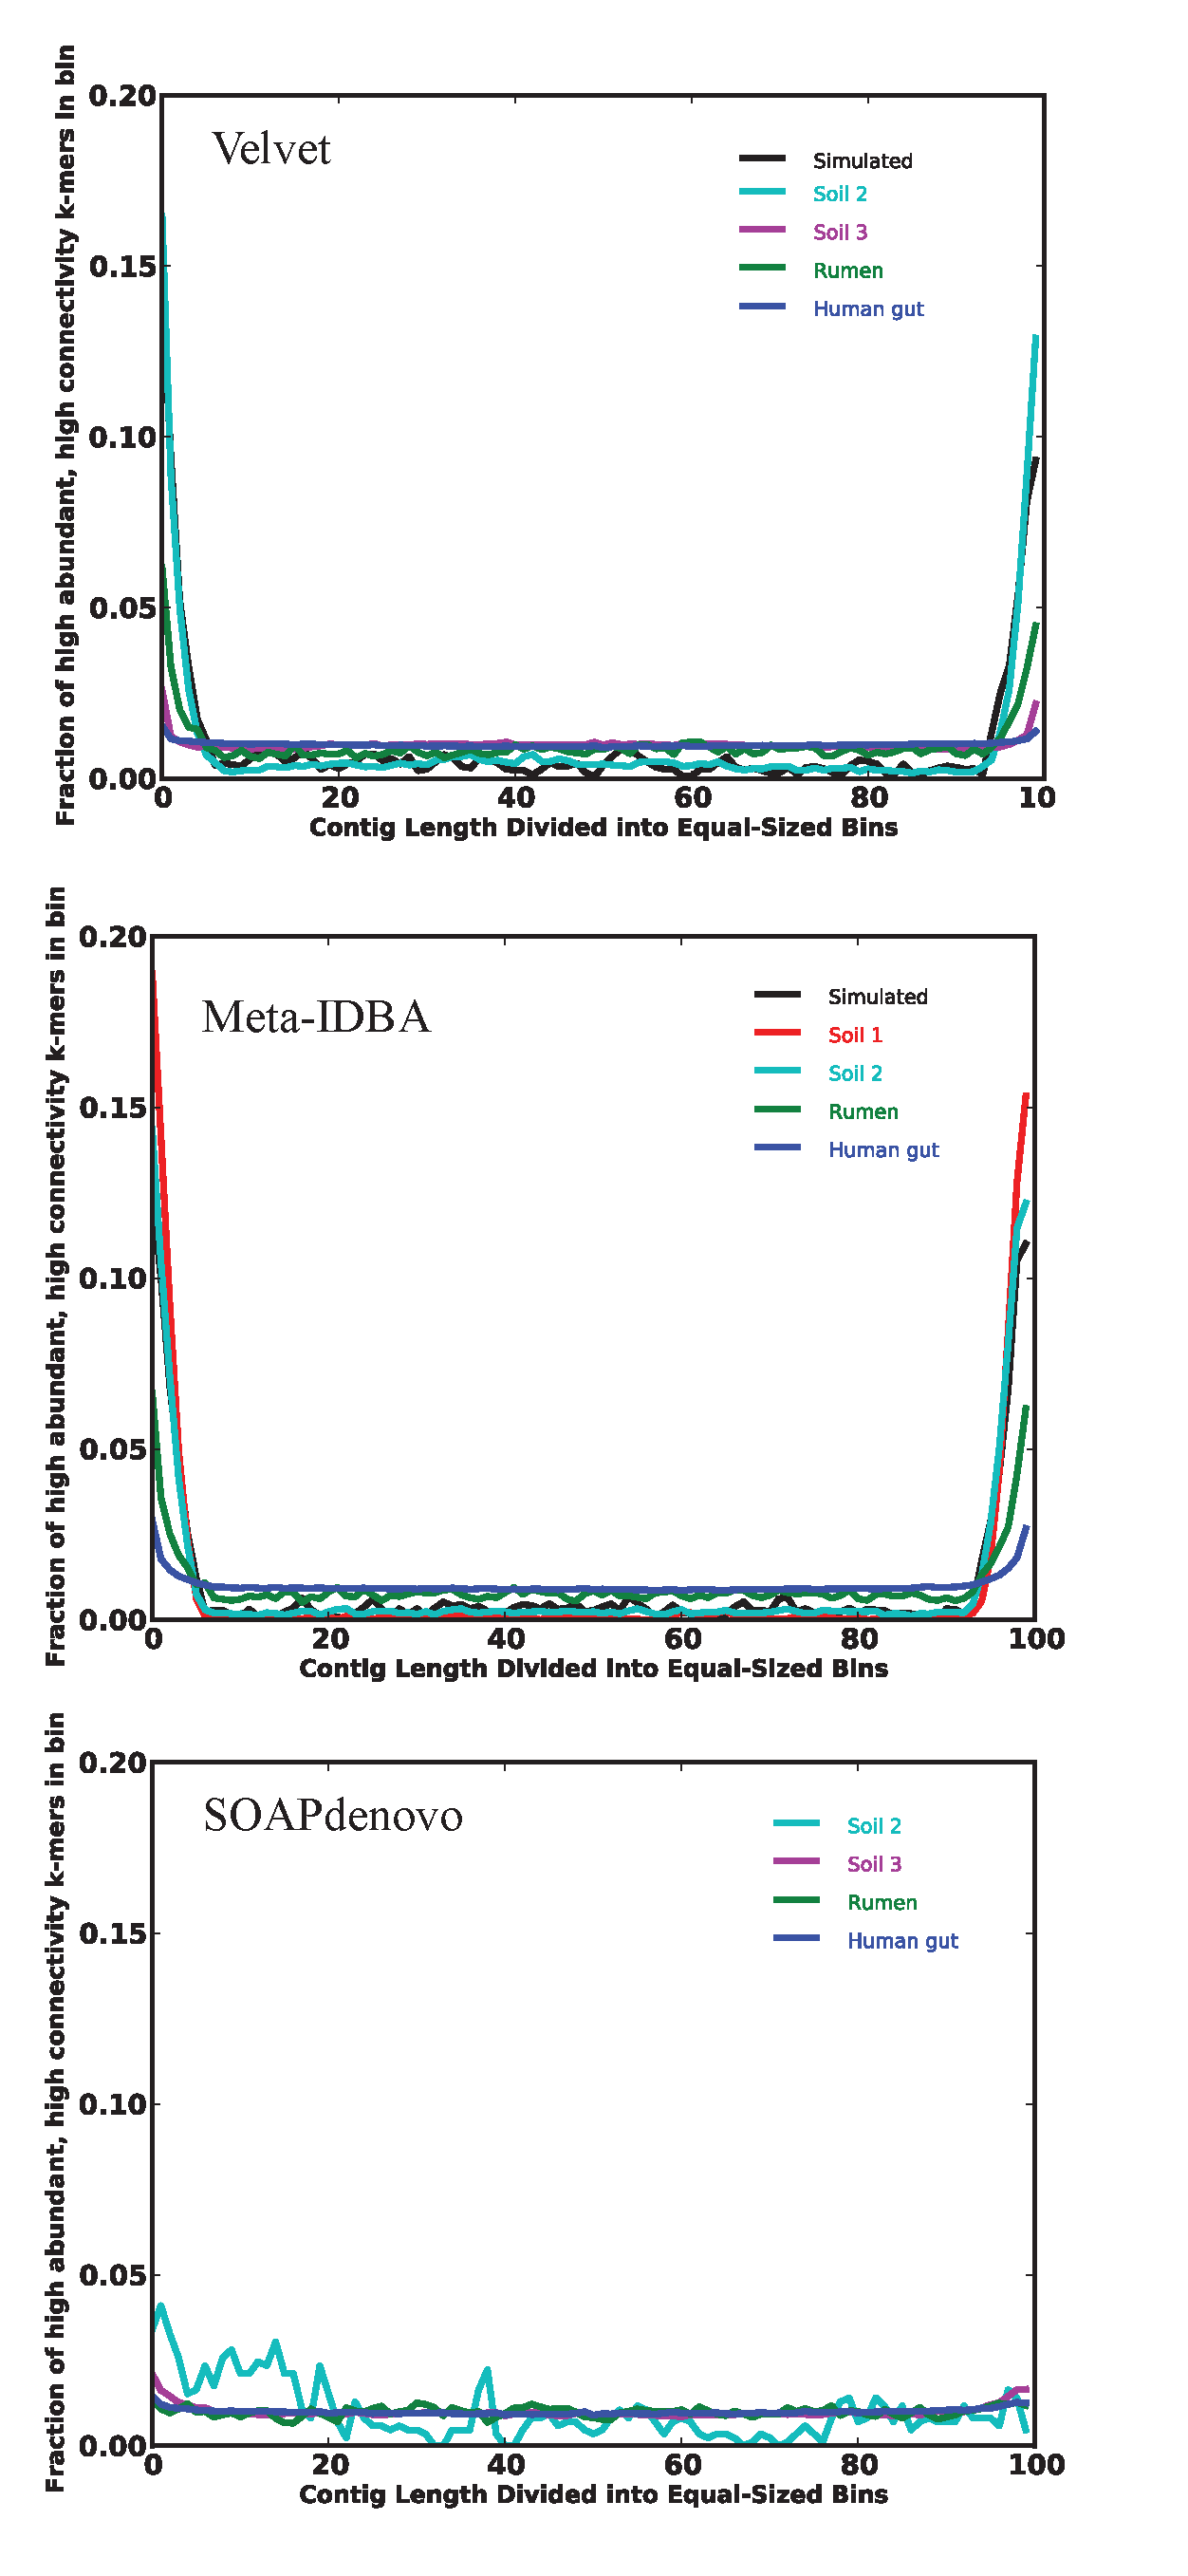
\includegraphics[width=\textwidth,height=\textheight5in,keepaspectratio]{./Figures/figure3-contigs.pdf}}
\caption{When incorporated into an assembly, abundant (greater than 50 times), highly-connecting sequences (k-mers) were disproportionately present at the ends of contigs.  The total fraction of highly-connecting k-mers which are incorporated into each contig binned region.}
\end{figure}

\begin{figure}
\center{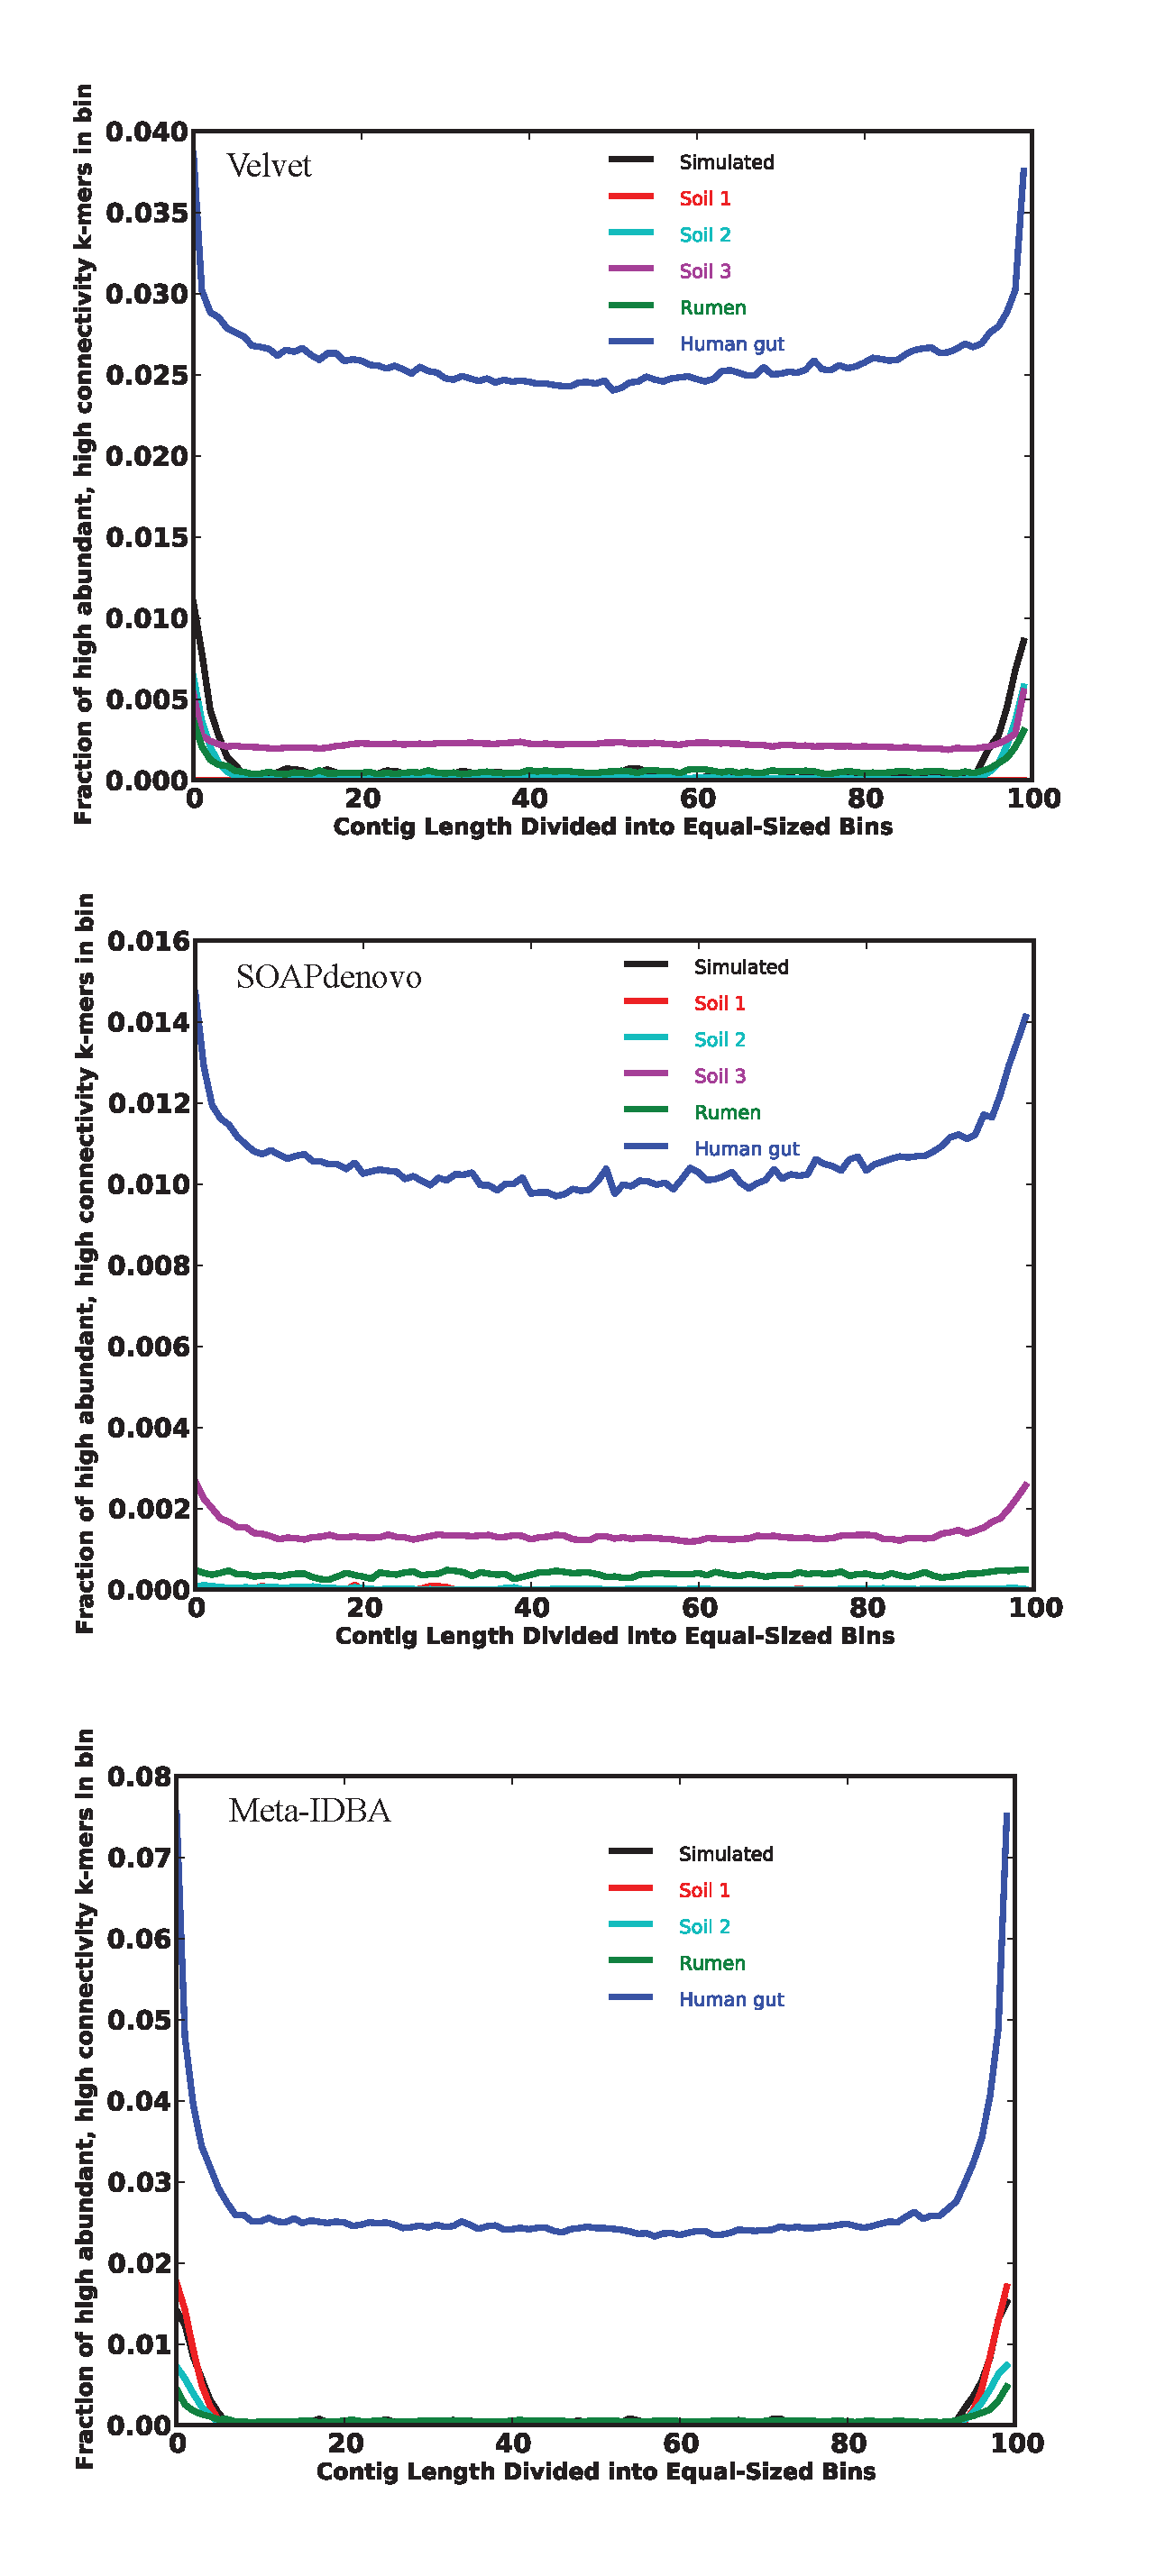
\includegraphics[width=\textwidth,height=\textheight5in,keepaspectratio]{./Figures/figure4-contigs.pdf}}
\caption{When incorporated into an assembly, abundant (greater than 50 times), highly-connecting sequences (k-mers) were disproportionately present at the ends of contigs.  The total fraction of all k-mers which are identified as high abundant, high connective sequences and incorporated into each contig binned region is shown.}
\end{figure}

\end{document}









